\section{Control System}\label{Control}
The goal of having a prosthesis is to make the life of the user  more convenient. Since the solution with the most notable potential to improve the users' life is an electric prosthesis a question comes to mind. How should such a prosthesis be controlled by the user, in order to reach a viable solution? 
Norman S. Nise define a control system in his book Nises' Control System Engineering and provides 4 reasons to use a control system
\begin{displayquote}
 \textit{"A control system consist of subsystems and processes assembled for the purpose of obtaining a desired output with desired performance given a specific input\\[...]\\ We build control systems for four primary reasons. 
\begin{enumerate}
    \item Power amplification
    \item Remote control
    \item Convenience of input form
    \item Compensation of disturbances "
\end{enumerate}}\hspace{0.65\textwidth} -Norman S. Nise \cite{Nise}
\end{displayquote} \label{Quote1}
\noindent The need of a control system is evident in this project. The control of a prosthesis allows compensation for the missing limb. Since the input can be selected by convenience, the project can choose any interface. There are many different kinds of control systems, an elaboration of which is used in this project can be seen in Chapter \ref{ch:Design} describing the design of the system. 
\subsection*{Interfaces}
The use of a control system allows for any input. It is therefore relevant to look into different interfaces that can be used to control the manipulator:

\subsubsection*{Surface electromyography}\label{sEMG}
sEMG or surface electromyography, is a way of interpreting the signals given when muscular activities occur. sEMG signals can be read by applying electrodes to the muscle, when the muscle contracts, a signal is sent through the electrodes and then analysed in the application used on the device reading it.\\
In Figure \ref{fig:sEMG}, the sinoid wave read from the sEMG, and the characteristics of it is shown 

\begin{figure}[H]
    \centering
    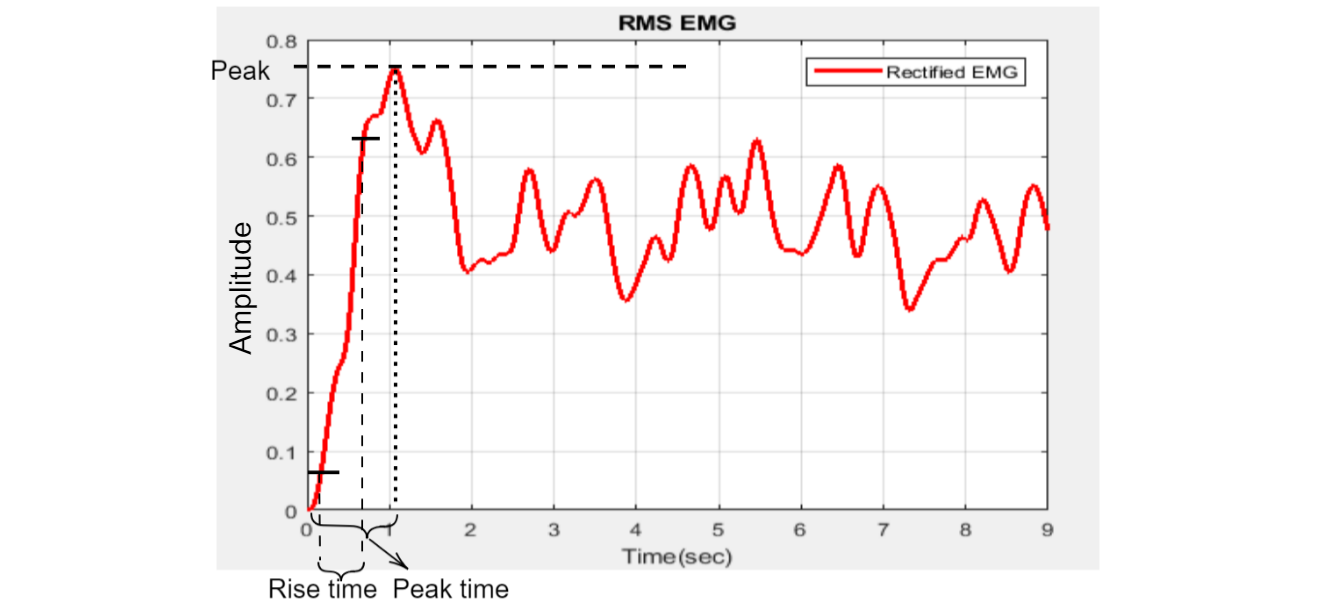
\includegraphics[width=12cm,height=7cm]{Figures/EMG/RPPT.png}
    \caption{The sinoid wave read from the sEMG, with the characteristics amplitude,  rise-time, peak and peak-time\cite{EMGDATA}}
    \label{fig:sEMG}
\end{figure}

\begin{itemize}
  \item \textbf{Amplitude} determines how intense your muscle contracts.
    \item \textbf{Peak} determines the maximum value in the signal.
    \item \textbf{Peak Time} is the time it take to reach maximum value.
    \item \textbf{Rise Time} is a measurement to determine a rise in the wave, from 10 percent to 90 percent of the final value.
    \item \textbf{Duration} can be described as the time it takes for a single oscillation of the sin-wave.
\end{itemize}

Some of the benefits to controlling a system with a sEMG is the ease of use, it is a non invasive system and depending on the programming the system can be fairly intuitive to use, while still be easy to equip. 
There are some downsides though, one being the noise of the data-stream. This control method requires the need of filters to interpret the inputs into usable data. Another is the need for a skintight seal on the muscle which can result in several difficulties see section \ref{Difficoulties}.

\subsubsection{Accelerometers}
Accelerometers measure the acceleration of gravity, which is measured in $m/s^2$ or g-force, with this information the orientation of the accelerometer can be calculated.\\
Systems such as the Inertial Measurement Unit(IMU) uses a combination of sensors such as accelerometers and gyroscopes to detect changes in roll, pitch and yaw and in linear acceleration\cite{IMUWorki40:online}.\\ These are often used in planes and ships and can be used as inputs in a controller\\ 
A good way to imagine a accelerometer is to imagine a ball with walls for directions, as seen in figure \ref{fig:spring}. E.g when the accelerometer is moved up the ball will move towards Z-, which means its an upward acceleration.\\
Most accelerometers is implemented with a spring attached to a ball that pressures a certain mass to measure the g-force and direction. 
\begin{figure}[H]
 \centering
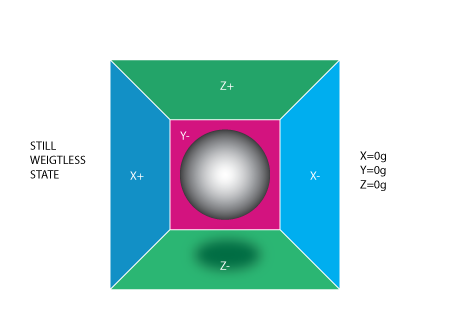
\includegraphics[width=8cm]{Figures/Technical_figures/spring.png}
 \caption{An accelerometer can be illustrated as a ball suspended in a room. If the ball touch one of the walls the devise is accelerating in the opposite direction of that wall. \cite{Gyroskop}}
 \label{fig:spring} 
\end{figure}

This method have similar benefits to the sEMG, its small and easy for the user, but the signal needs processing to be interpret.
\\ 
\subsubsection*{Eye-tracking}
Eye tracking is a devise used to interpret where the gaze of the user is directed. 

\begin{figure}[H]
    \centering
    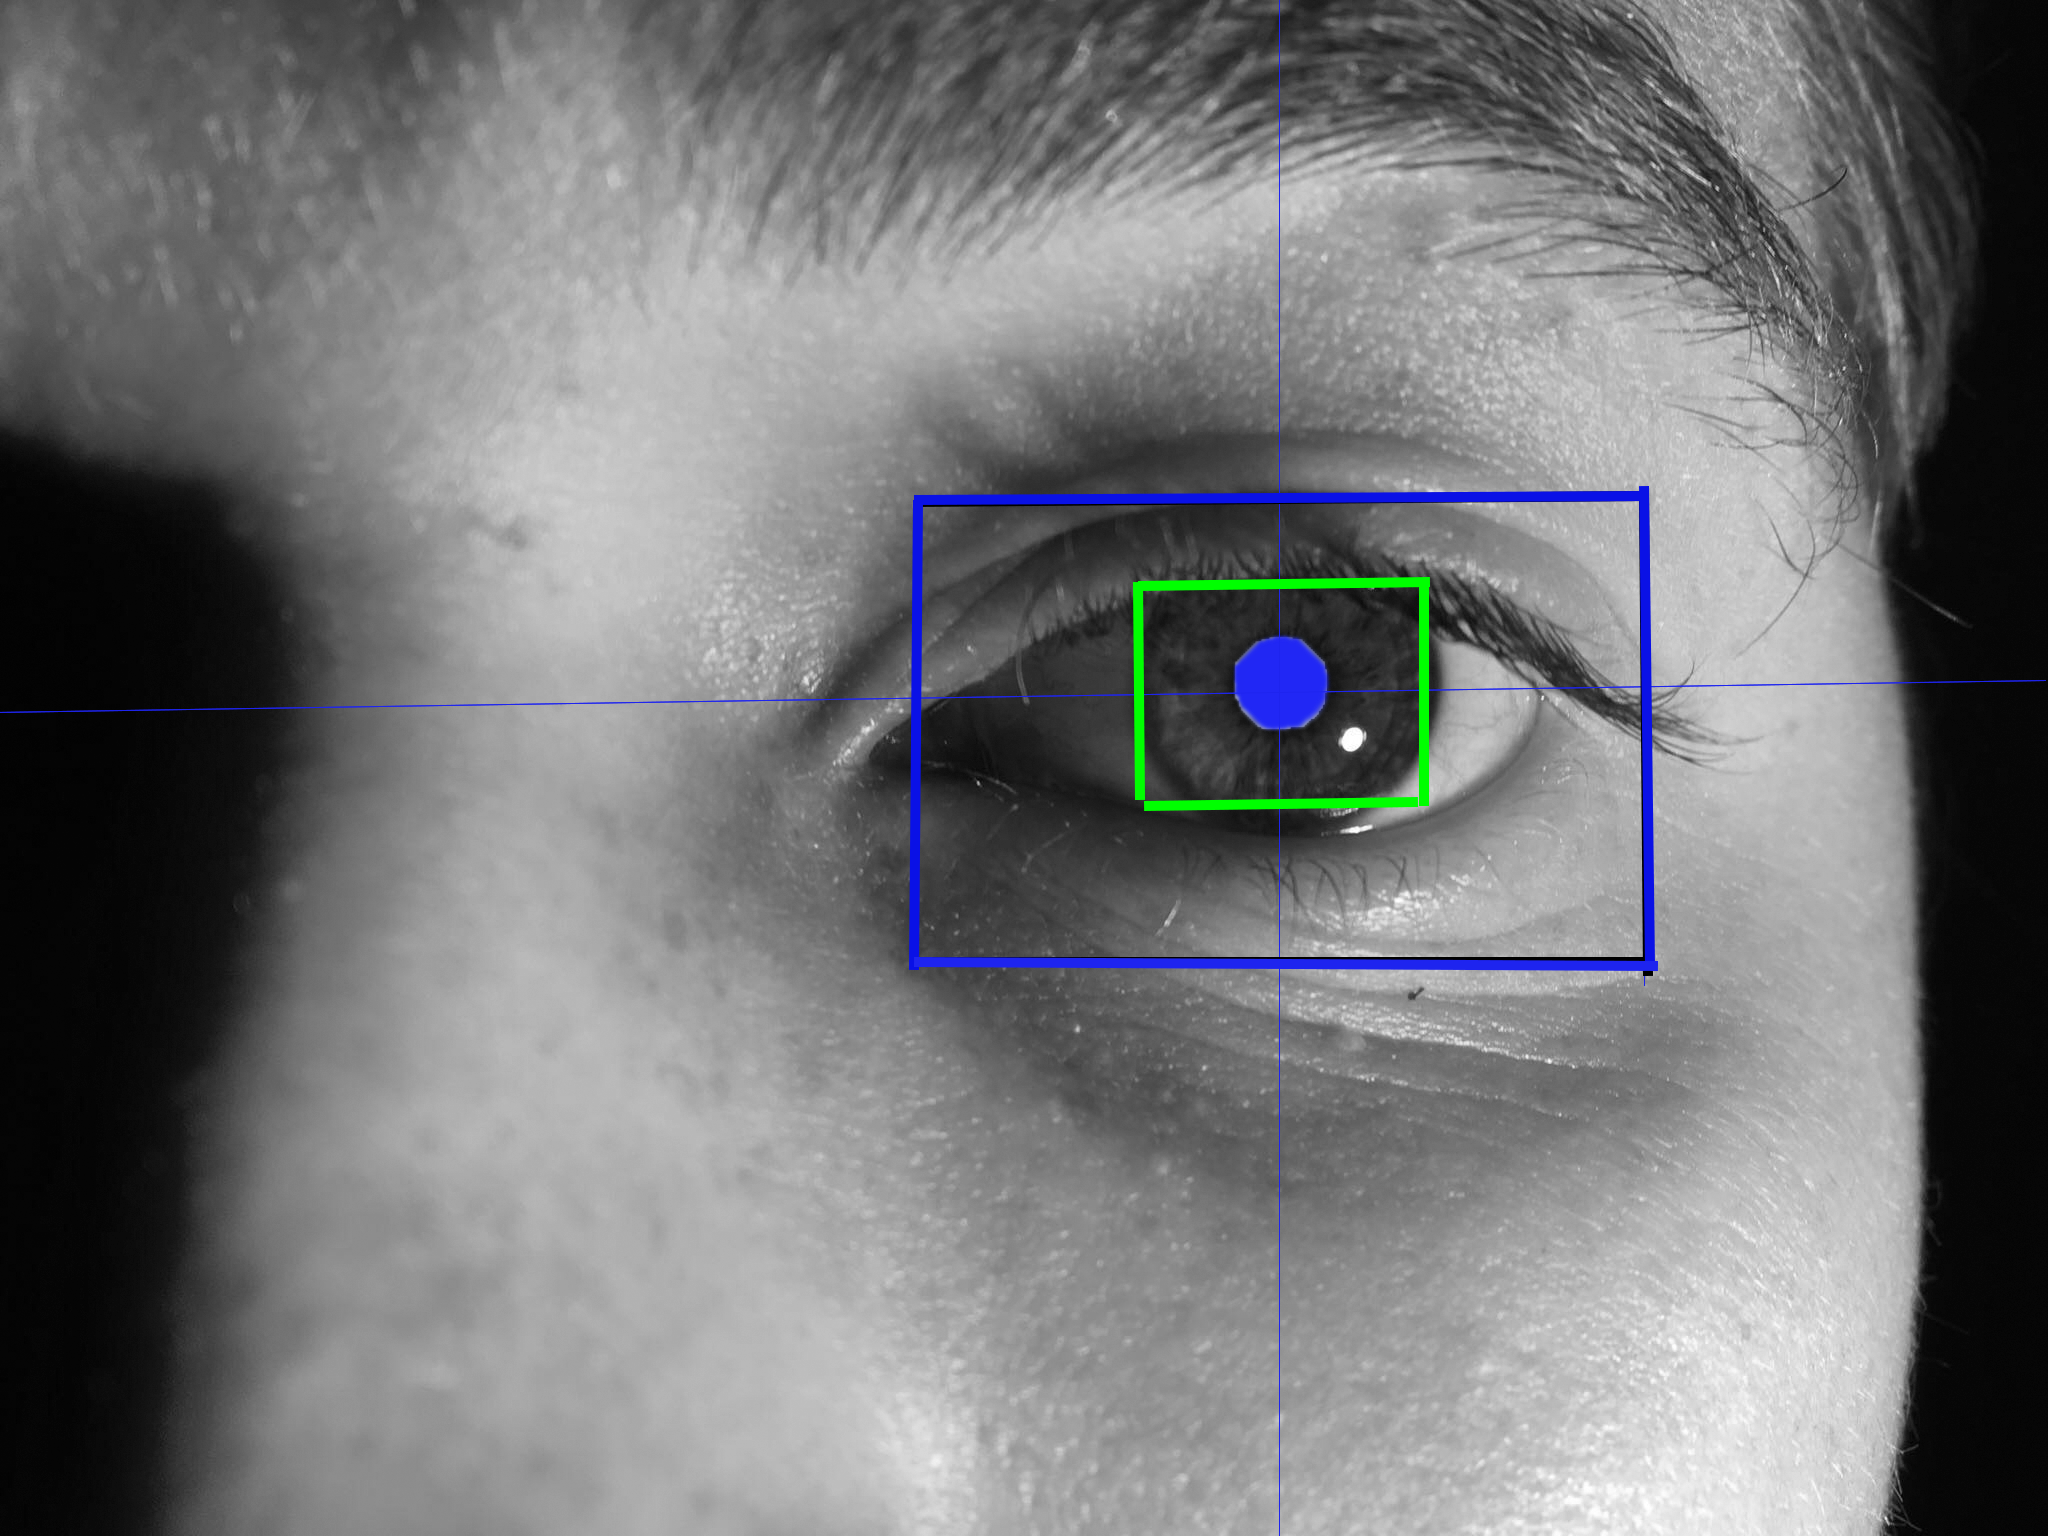
\includegraphics[width=10cm,height=7cm]{Figures/Contextual_figures/eye-tracking.png}
    \caption{An illustration on what is seen by Eye-tracking the users pupil is illuminated by infrared light which can then be used to as a control input}
    \label{fig:Eye}
\end{figure}

As seen in figure \ref{fig:Eye}, the devise will project  a dim infrared light into the users pupil. When the pupil is illuminated by light a infrared camera will catch the movement of the reflection and send the data to the device which will use it to measure where the user is looking.\\
These features could be used to steer the arm towards desirable locations relying solely on eye-tracker \cite{EyeTrack}. There are some clear disadvantages to this interface. The device has to detect the eye movement, meaning that the ideal position is in front of the users face. There is also a chance of false positives where the user does not want to move the arm bur a sudden movement makes the user look in another direction causing the arm to move. 

\subsubsection*{Joystick}
A joystick can be used to control many things, such as wheelchairs, computers and many other devices. A joystick works through the use of potentiometers. A potentiometer is a variable resistor, when the joystick is moved in one direction, the resistances will change and the voltage drop over potentiometer changes. The voltage drop can use be to translate in to a control signal for the device it is used on. Some joysticks is made in combination with a sip and puff system\cite{Jouse}. A joystick i often used for a person how are in a wheelchair or have minimal to no motor coordination.\\ 
\begin{figure}[H]
    \centering
    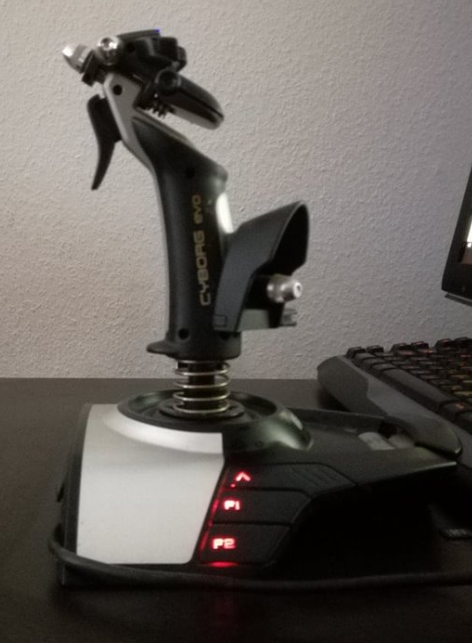
\includegraphics[width=5cm,height=7cm]{Figures/Contextual_figures/Joystickl.jpg}
    \caption{An illustration of a joystick which can be used as a control input}
    \label{fig:picjoystick}
\end{figure}
The joystick mainly has two disadvantages. First of all it requires an arm to move. It is more convenient for the user to use the functional arm to do the movement rather than using the joystick thus making the interface redundant. Secondly, prolonged use of a joystick can also lead to repetitive strain injuries. 
\subsubsection*{Sip-and-puff}
The sip and puff drive system use one or more pressure differential sensors. The User sip or blows through one straw and onto pressure differential sensors. Depending on the sip and puff system and the way they are configured, some systems is only made for puff and sip where others can differentiate a slow sip or puffs from a hard sip or puffs. This all depends on the use of this system, it can be used on its own or in combination with others control systems\cite{Snp}. Most users for this system is wheelchair users like paraplegics or people with multiple scleroses.\\
\begin{figure}[H]
    \centering
    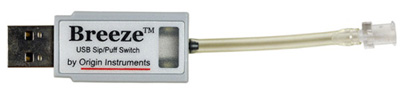
\includegraphics[width=9cm,height=3cm]{Figures/Contextual_figures/breeze_400.jpg}
    \caption{a photo of the Breeze sip-and-puff input devise. This photo was provided in courtesy of Origin Instruments \ref{st:Origin}\\ 
    Sip/Puff Breeze 400\cite{Snp}}
    \label{fig:Sip/Puff}
\end{figure}
The disadvantages of this system is the placement of the interface. The user cannot talk while operation the prosthesis. 
\subsubsection*{I-tongue control system}
Thanks to the ever shrinking sizes of electronics, it is now possible to have a control system within the mouth in form of a retainer. The I-tongue control system from TKS\cite{TKS}, consists of two control areas one is a keyboard with 10 buttons, used as the "old mobile phone" where one button containing three or more letters and characters, the other control area on the I-tongue is a mouse pad, furthermore the user can select different control modes. A piercing is placed through the tongue of the user. When the user moves the piercing over the sensor, the signal for the sensor is transmitted through a wireless signal. The signal can be used to control almost any device. This is mostly used for tetraplegics or people with muscular failure like ALS\cite{TDSp}.\\
\begin{figure}[H]
    \centering
    \includegraphics[width=12cm,height=7cm]{}
    \caption{A view of how user could use the tongue to control a device\cite{TDSp}}
    \label{fig:TDS}
\end{figure}
 
\subsubsection*{Safety precautions}

One way to ensure safety for the user, is to isolate the controller from the prosthesis, so if there is a short-circuit within the prosthesis, the user do not have to fear for any electrocution from the power source. This separation can be done in many ways, some is to use an isolating transformer\cite{isotrans} or through the use of a wireless signal like Bluetooth.  \\
Another way to ensure some safety for the user, is to keep the forces of prosthesis minimised to a non-harmful level. Equations has been done to measure how much force a human can resist, as seen in "pdf- med force".\\  

\section{Summary} %Both prosthesis and control system 
Different viable options of prosthesis' and control systems has been presented in the chapter above. By investigating these options an understanding of existing solutions and viable system-controls can be reached.\\
Certain safety measures has been reviewed and a sub-conclusion has been taken into consideration. 